\documentclass[a4paper,12pt]{article}
\usepackage[utf8x]{inputenc}
\usepackage[T1]{fontenc}
\usepackage[english, ngerman]{babel}
\usepackage{listings}
\usepackage{graphicx}
\usepackage{ulem}
\newtheorem {Bsp}{Beispiel}[section]

\usepackage{xcolor}
\colorlet{punct}{red!60!black}
\definecolor{background}{HTML}{EEEEEE}
\definecolor{delim}{RGB}{20,105,176}
\colorlet{numb}{magenta!60!black}
\newenvironment{simplechar}{%
	\catcode`\$=12
	\catcode`\&=12
	\catcode`\#=12
	\catcode`\^=12
	\catcode`\_=12
	\catcode`\~=12
	\catcode`\%=12
}{}
\lstdefinelanguage{json}{
	basicstyle=\normalfont\ttfamily,
	numbers=left,
	numberstyle=\scriptsize,
	stepnumber=1,
	numbersep=4pt,
	showstringspaces=false,
	breaklines=true,
	frame=lines,
	backgroundcolor=\color{background},
	literate=
	*{0}{{{\color{numb}0}}}{1}
	{1}{{{\color{numb}1}}}{1}
	{2}{{{\color{numb}2}}}{1}
	{3}{{{\color{numb}3}}}{1}
	{4}{{{\color{numb}4}}}{1}
	{5}{{{\color{numb}5}}}{1}
	{6}{{{\color{numb}6}}}{1}
	{7}{{{\color{numb}7}}}{1}
	{8}{{{\color{numb}8}}}{1}
	{9}{{{\color{numb}9}}}{1}
	{:}{{{\color{punct}{:}}}}{1}
	{,}{{{\color{punct}{,}}}}{1}
	{\{}{{{\color{delim}{\{}}}}{1}
	{\}}{{{\color{delim}{\}}}}}{1}
	{[}{{{\color{delim}{[}}}}{1}
	{]}{{{\color{delim}{]}}}}{1},
}

\begin{document}
	\title{Extraktion und Erweiterung eines Knowlegde Graphen für Publikationen und Zitationen}
	\author{Timo Stroick}
	\maketitle
	\tableofcontents
	\section{Einleitung}
	Weltweit werden in fast allen Programmen die wir Alltäglich benutzen Datenbanken verwendet. Sei es unsere Freundesliste, eine Website und sogar beim Einkaufen überall treffen wir auf sie. Es gibt viele Formen von Datenbanken wie zum Beispiel relationale, hierarchische, objektorientierte Datenbanken und noch viele mehr. In dieser Bachelorarbeit wird ein Knowlegde Graph in eine relationale Datenbank umgewandelt und anschließend noch mit einem weiteren Graphen erweitert. Dabei stellt sich natürlich die Frage was ist ein Knowledge Graph überhaupt. Grundsätzlich ist es auch eine Form von Datenbank. Man kann sich die Datenbank am besten so vorstellen das man Daten so speichert das man sie leichter suchen kann. Deshalb werden Daten meist mit Themen Gebieten zusammen verbunden. Wie bei Suchmaschinen wird mit einem Schlüsselwort gesucht und in dieser Art von Datenbank stehen alle Daten die etwas damit zu tun haben in direkter Verbindung mit dem Schlüsselwort. So lässt es sich einfacher und schneller in der Datenbank suchen. Im Gegensatz dazu steht eine relationale Datenbank in die der Knowledge Graph eingefügt wird. Hierbei steht nicht das suchen im Vordergrund sondern in welcher Beziehung die Daten zueinander stehen. Damit ist der Grundaufbau sehr Unterschiedlich und das ist die Aufgabe die es gilt zu überwinden. Die Knowlegde Graphen die benutzt werden sind der Microsoft Academic Knowledge Graph und das Digital Bibliography \& Library Project (DBLP) der Universität Trier. Beide Graphen beinhalten Publikationen, Facharbeiten, Konferenzen und Fachbücher. Die Universität Trier beinhaltet nur Daten im Bereich der Informatik was die Daten Anzahl um einiges verringert. Hier sind nur grob 5,2 Millionen Publikationen vertreten. Im Gegensatz da zu hat der Microsoft Academic Knowledge Graph keinen Fachbereich und ist international Vertreten. Daraus ergeben sich dann die 209,7 Millionen Publikationen in der Datenbank und das alleine im Jahre 2018. Für den ersten Teil werden die DBLP Daten in ein relationale Datenbank eingefügt. Dafür wird eine Datenbank entwickelt und anschließend alle Daten einzeln extrahiert und gespeichert. Dies machen wir mit der DBLP da es zunächst weniger Daten sind und in der DBLP keine richtigen Zitate vorhanden sind. Der zweite Teil ist nun das erweitern. Hier wird der Microsoft Academic Knowledge Graph verwendet da er zu den ganzen Publikationen auch noch 146 Millionen Zitation enthält. Für diesen Zweck erhält die Datenbank zusätzlich eine Zitat Relationen wo die Daten eingefügt werden können. Vorher werden zunächst die richtigen Überschneidungen gefunden damit die richtigen Daten eingefügt werden.
	
	\section{Extraktion}
	Kommen wir nun zum ersten Teil, die Extraktion. Dafür gucken wir uns zunächst die Daten an welche wir Extrahieren werden. Die DBLP bietet dafür 2 Möglichkeiten an. Die erste ist eine Request API oder auch Schnittstelle an. Das heißt man kann über eine Request, also über eine Anfrage, an den Server der DBLP Daten erhalten. Es ist also Möglich eine Anfrage zustellen die alle Autoren die mit A anfangen anfragt. Für unseren Fall ist die zweite Möglichkeit besser geeignet. Denn hier bekommt man ein Dump File welches dblp.xml heißt. Ein Dump File ist ein Ausdruck von dem gesamten Inhalt eines Speichers in dem Fall von einer Datenbank. Das File enthält alle Daten die die Datenbank zu dem Zeitpunkt besitzt. Da sich die Datenbank regelmäßig erweitert oder ändert, erstellt die DBLP regelmäßig neue Dump Files. Das File was benutzt wird ist vom 13.05.2020. Es kann viele Dateiformate haben, aber in diesem Fall ist es im XML-Format. Hierzu gibt es eine Dokumentation die die Formatierung des XML-Formates beschreibt. Da diese schon "DBLP - Some Lessons Learned" heißt lässt es darauf schließen das einige Fehler bei dem Ursprünglichen Design aufgetreten sind und einige Änderungen gemacht wurden. Die erste Dokumentation der DBLP ist vom 18. Juni 2009. Zu dem Zeitpunkt waren nur 532MB in der XML-Datei. Im Gegensatz da zu sind jetzt 2.806MB in der Datei also schon das 5-Fache der Ursprünglichen Datei. Durch das Wachstum wurden einige Anpassung getätigt die von der Dokumentation abweichen. So mit muss die Formatierung der Datenstrukturen an Hand der Datei selber Herausgefunden werden. 
	
	Für das Extrahieren der Daten wird dann ein Parser benötigt der die XML-Datei ausliest. Denn für die meisten Parser sorgt eine Datei dieser Größe zu Problemen. Daher wird ein eigener Parser geschrieben um dieses Problem zu umgehen. Durch die Dokumentation erfahren wir das es nur eine bestimmte Anzahl an Tags gibt die verwendet werden.
	\begin{center}
		<!ELEMENT dblp (article|inproceedings| proceedings|book|incollection|phdthesis|mastersthesis|www)*>
	\end{center}
	
	Das ist ein Ausschnitt aus der Dokumentation und beschreibt alle Elemente(Tags) die nur auftreten sollen. Nach dem Testen traten auch keine anderen Elemente auf. So werden die benötigten Fähigkeiten die der Parser haben muss limitiert.
	
	\subsection{Parser}
	Um mit der Erklärung des Parsers anzufangen müssen wir erst das Dateiformat XML weiter ausführen. XML heißt Extensible Markup Language und ist eine Auszeichnungssprache mit deren Hilfe man Daten im Textformat speichern kann. Es funktioniert so das man mit einem Tag einem bestimmtem Element einen Namen oder eine Kategorie zuteilen kann z.b '<author> Timo Stroick </author>'. Hierbei ist Alles zusammen ein Element und das eingeklammerte "author" ein Tag. Dabei ist darauf zu achten das man Elemente immer mit dem dazugehörigen Endtag schließen muss wie im Beispiel schon gezeigt. Eine weitere Möglichkeit ist Elemente in Elemente zu schreiben. Hier gibt es eine Besondere Regel die XML ausmacht. Denn Elemente die in anderer Elemente geschrieben sind müssen erst geschlossen werden bevor die äußeren geschlossen werden dürfen. Durch diese Regeln entsteht die Typische hierarchische Struktur des XML Dateiformats. In der dblp.xml sind alle Daten in ein Tag eingeschlossen das dblp heißt. So fängt die Datei bei <dblp> an und enden bei </dblp>. Damit sind alle wichtigen Daten zwischen den beiden Tags. 
	
	\begin{figure}[!htb]
	\lstset{language=XML}
		\begin{lstlisting}
<article mdate="2020-03-12">
	<author>Moritz Lipp</author>
	<author>Michael Schwarz 0001</author>
	<author>Daniel Genkin</author>
	<title>Meltdown</title>
	<journal>meltdownattack.com</journal>
	<ee>meltdownattack.com/meltdown.pdf</ee>
	<year>2018</year>
</article>
	\end{lstlisting}
	\caption{xml-Ausschnitt}
	Ein Beispiel Ausschnitt wie ein typischer Eintrag in der dblp.xml aussieht. Dieser wurde verkürzt und angepasst.
	\end{figure}
	
	Der Parser ist in einer eigene Klasse. Um nun mit dem Parser anzufangen lesen wir die Daten Zeilenweise in der Klasse ein um das Problem mit der Dateigröße zu umgehen. Denn würde man alles auf einmal einlesen würde der Speicher des Programms schnell voll werden und damit das Programm überlasten. Nun checken wir in den Zeilen nach den Tags. Wenn wir ein Tag gefunden haben überprüfen wir dessen Namen und reagieren mit einem bestimmten Fall. Da wir durch die Dokumentation alle Tags kennen, die in der 2. Hierarchie auftreten können, wissen wir das nur 8 Fälle behandelt werden müssen. Somit haben wir nur 8 Methoden mit denen wir jeden Fall abdecken. Jede Methode liest weiter Tags ein bis das Endtag die Methode beendet. Das zählt natürlich auch für das dblp-Endtag welchen den Parser beendet. Die nun eingelesenen Elemente in der 3. Hierarchie sind die Daten des entsprechenden Elements wie zum Beispiel bei 'article' könnte es der Author sein der eingelesen wird. Die Daten werden nun in eine weitere Klasse übergeben und dort den richtigen Entitäten zugewiesen. Denn die 8 Elemente der XML-Datei sind nicht die Entitäten die wir in der Datenbank benutzen. Wir wollen die Datenbank so Allgemein gültig halten wie möglich. Zum Schluss wird in der letzten Klasse die Daten nur noch in die Datenbank eingefügt. Alle Klassen folgen dem Single Responsibility Principle dieses besagt das jede Klasse nur eine Aufgabe verfolgt. Dem nach extrahiert die Parser-Klasse die Daten , die Funktionen-Klasse teilt die Daten in die Entitäten auf und die Insert-Klasse fügt die Daten in die Datenbank ein. So ist das Programm einfacher nachzuvollziehen für Leute die sich noch nie damit auseinander gesetzt haben. Und es gibt ein sauberes Programmbild ab.
	
\begin{figure}[!htb]
	\centering
	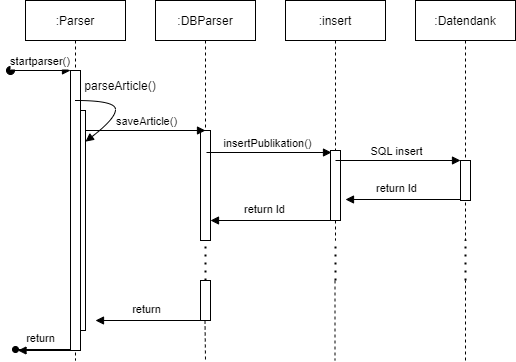
\includegraphics[width=10cm,keepaspectratio]{SequenzDiagramParser}
	\caption{Sequenzdiagramm-Auschnitt}
	\label{fig:sequenzdiagramm}
\end{figure}
	
	In Abbildung \ref{fig:sequenzdiagramm} sehen wir einen Typischen Programmablauf vom Parser. In diesem Beispiel Ablauf wird ein 'article' Element eingelesen. Zu nächst wird die Parser-Klasse mit der startParser-Funktion in der Main-Methode aufgerufen und liest ein Tag nach dem anderen bis er auf einen Treffer stößt. In diesem Fall ist es das Tag 'article' ein Treffer. Nun wird die parseArticle-Methode in der selben Klasse aufgerufen. In der Methode werden nun die weiter folgenden Elemente ausgelesen und deren Daten zwischengespeichert. Dies geschieht solange bis das Endtag von 'article' wieder eingelesen wird. Jetzt werden alle Daten and die saveArticle-Methode der Funktionen-Klasse übergeben. In dieser Klasse werden nun die Daten an die Datenbank angepasst. Denn in der Datenbank gibt es keine Entität die Artikel heißt. Das wird erst im nächsten Abschnitt erklärt. Im Allgemeinen wird der Artikel dann in Publikation, Autoren, elektronische Version und Fachzeitschrift zerteilt und noch in die Beziehungen zwischen den Entitäten. Da die Daten nun richtig Zerlegt sind werden sie an die Insert-Klasse übergeben. Das geschieht über die insertPublikation-Methode. Jetzt haben wir alle Daten und haben sie richtig zugewiesen. Daraufhin werden sie mit SQL in eine Postgres Datenbank gespeichert. In der Methode ist drauf zu achten das nur triviale SQL Befehle benutzt werden und keine Speziellen Befehle eines Datenbank Types. Deshalb beschränke ich mich auf Insert-Befehle und Select-Abfragen. Schlussendlich gebe ich denn Primärschlüssel der Publikation zurück um die Beziehungen zwischen den Entitäten in der Datenbank einzutragen. Wenn nun die saveArticle-Methode zu ende läuft und sich erfolgreich beendet, sucht die startparser-Methode nach dem nächsten Tag. So wird jedes Element nacheinander in die Datenbank eingespeichert bis das Endtag von dblp eingelesen wird.

	\subsection{Datenbank}
	Zur Erstellung der Datenbank gucken wir uns zunächst die Daten an. Die DBLP gibt uns schon mit den 8 Tags(article, inproceedings, proceedings, book, incollection, phdthesis, mastersthesis, www) einen groben Überblick. Nur diese Tags sind noch nicht in dem relationalen Datenbanken Format. Deshalb werden diese Tags nochmal in kleinere Entitäten teilen. Zunächst werden wir die Begriffe ein wenig klarer stellen. Ein 'article' ist ein Artikel oder auch eine Publikation in einer Fachzeitschrift. 'proceedings' ist in diesem Zusammenhang eine Konferenz die gehalten wurde und dazu passten sind 'inproceedings' Puplikationen die zu dieser Konferenz gehören. Zum Ende ist 'incollection' eine Publikation in einem Buch. Die Restlichen sind sehr wahrscheinlich selbst erklärend. Daraus ergeben sich dann diese Entitäten Author, Publikation, Homepage, Konferenz, Fachzeitschrift, Buch, elektronische Version, ISBN, Herausgeber und deren Beziehungen. Hier durch erhalten wir dann dieses ER Modell.
	
	\subsubsection{ER Modell}
	\begin{figure}%[!htb]
		\centering
		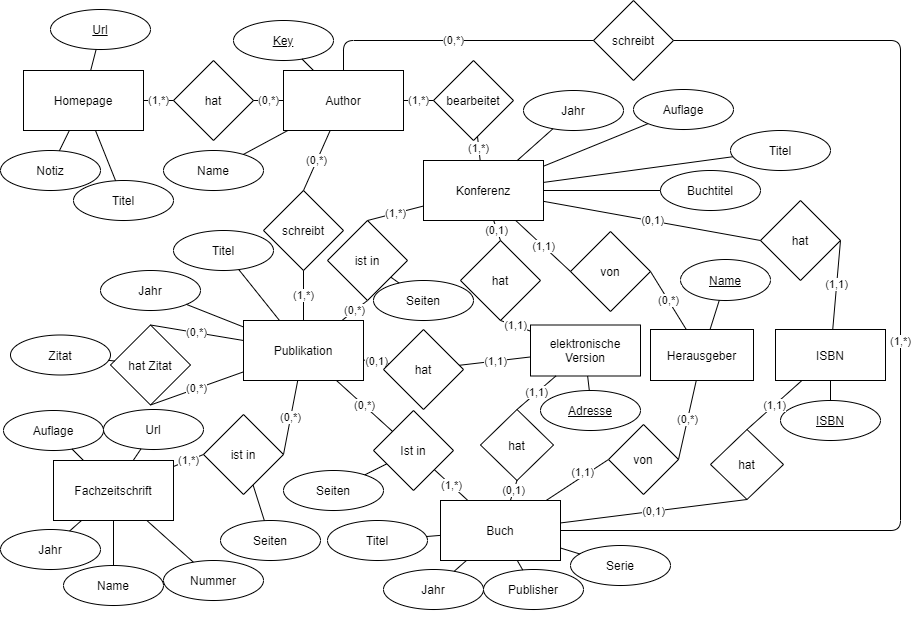
\includegraphics[width=14cm,keepaspectratio]{ER-Modell}
		\caption{ER-Modell}
		\label{fig:er-modell}
	\end{figure}

	Dieses Modell müssen wir nun Umwandeln. Da wir in der Datenbank nur Tabellen anlegen können müssen wir dieses ER-Modell in die Form von Tabellen bringen. Diese Form ist dann das Relationale Schema. Dieses Schema beschreibt genau das gleiche wie das ER-Modell.
	\subsubsection{Relationales Schema}
	\begin{simplechar}
		\begin{flushleft}

		\begin{small}
			Autor(\uline{Key}, Name) \newline
			Homepage(\uline{Url}, Titel, Notiz)\newline
			Publikation(\uline{Id}, Titel, Jahr, Universität)\newline
			Buch(\uline{Id}, Titel, Jahr, Serie, Auflage, Herausgeber)\newline
			Fachzeitschrift(\uline{Id}, Url, Name, Nummer, Auflage, Jahr, Herausgeber)\newline
			Konferenz(\uline{Id}, Titel, Buchtitel, Serie, Auflage, Jahr, Herausgeber)\newline
			elektronischeVersion(\uline{Adresse})\newline
			ISBN(\uline{ISBN})\newline
			Publikation_ist_in_Konferenz(\uline{\dotuline{PublikationId}, \dotuline{KonferenzId}},Seiten)\newline
			Publikation_ist_in_Fachzeitschrift(\uline{\dotuline{PublikationId}, \dotuline{FachzeitschriftId}},Seiten)\newline
			Publikation_ist_in_Buch(\uline{\dotuline{PublikationId}, \dotuline{BuchId}},Seiten)\newline
			Autor_bearbeitet_Konferenz(\uline{\dotuline{AutorKey}, \dotuline{KonferenzId}})\newline
			Autor_schreibt_Publikation(\uline{\dotuline{AutorKey}, \dotuline{PublikationId}})\newline
			Autor_schreibt_Buch(\uline{\dotuline{AutorKey}, \dotuline{BuchId}})\newline
			Autor_hat_Homepage(\uline{\dotuline{AutorKey}, \dotuline{HomepageUrl}})\newline
			Publikation_hat_Zitat(\uline{\dotuline{HatZitatKey}, \dotuline{IstZitiertKey}}, Zitat)\newline
			Konferenz_hat_elektronischeVersion(\uline{\dotuline{KonferenzId}, \dotuline{Adresse}})\newline
			Buch_hat_elektronischeVersion(\uline{\dotuline{BuchId}, \dotuline{Adresse}})\newline
			Publikation_hat_elektronischeVersion(\uline{\dotuline{PublikationId}, \dotuline{Adresse}})\newline
			Konferenz_hat_ISBN(\uline{\dotuline{KonferenzId}, \dotuline{ISBN}})\newline
			Buch_hat_ISBN(\uline{\dotuline{BuchId}, \dotuline{ISBN}})\newline
			\label{fig:relationalesSchema}
		\end{small}
	\end{flushleft}
	\end{simplechar}
	Das ist nun das ER-Modell genau übertragen ins Relationale Schema. Der erste Name ist der Name der Tabelle und alle Namen in der KLammer sind die Attribute in der Tabelle .Hier sieht man das auch Beziehungen zwischen den Entitäten eine eigene Tabelle bekommen. Denn so werden die Daten mit einander Verbunden. Die unterstrichenen Attribute stellen die Primärschlüssel da. Primärschlüssel sind Attribute womit man die Daten dieser Entität genau unterscheiden kann. Gibt es keine eindeutige Eigenschaft so erstellen wir einen künstlichen Schlüssel. In dem Fall heißen alle künstlichen Schlüssel Id. Die unterpunkteten Attribute sind Fremdschlüssel. Diese Schlüssel sind Primärschlüssel aus anderen Tabellen. Damit stellen sie eine eindeutige Verbindung zu anderen Entitäten her. Da hier noch einige überflüssige Tabellen enthalten sind werden die Tabellen verschmolzen.
	\subsubsection{Verschmolzenes Relationale Schema}
	\newpage
	\begin{simplechar}
		\begin{flushleft}
		\begin{small}
			Autor(\uline{Key}, Name)\newline
			Homepage(\uline{Url}, Titel, Notiz)\newline
			Publikation(\uline{Id}, Titel, Jahr, Universität)\newline
			Buch(\uline{Id}, Titel, Jahr, Serie, Auflage, Herausgeber)\newline
			Fachzeitschrift(\uline{Id}, Url, Name, Nummer, Auflage, Jahr, Herausgeber)\newline
			Konferenz(\uline{Id}, Titel, Buchtitel, Serie, Auflage, Jahr, Herausgeber)\newline
			elektronischeVersion(\uline{Adresse})\newline
			ISBN(\uline{ISBN}, \dotuline{BuchId}, \dotuline{KonferenzId})\newline
			Publikation_hat_Zitat(\uline{\dotuline{HatZitatKey}, \dotuline{IstZitiertKey}}, Zitat)\newline
			Autor_hat_Homepage(\uline{\dotuline{AutorKey}, \dotuline{HomepageUrl}})\newline
			Autor_bearbeitet_Konferenz(\uline{\dotuline{AutorKey}, \dotuline{KonferenzId}})\newline
			Autor_schreibt_Publikation(\uline{\dotuline{AutorKey}, \dotuline{PublikationId}})\newline
			Autor_schreibt_Buch(\uline{\dotuline{AutorKey}, \dotuline{BuchId}})\newline
			Publikation_ist_in_Konferenz(\uline{\dotuline{PublikationId}, \dotuline{KonferenzId}}, Seiten)\newline
			Publikation_ist_in_Fachzeitschrift(\uline{\dotuline{PublikationId}, \dotuline{FachzeitschriftId}}, Seiten)\newline
			Publikation_ist_in_Buch(\uline{\dotuline{PublikationId}, \dotuline{BuchId}},Seiten)\newline
			Publikation_hat_elektronischeVersion(\uline{\dotuline{PublikationId}, \dotuline{Adresse}})\newline
			Buch_hat_elektronischeVersion(\uline{\dotuline{BuchId}, \dotuline{Adresse}})\newline
			Konferenz_hat_elektronischeVersion(\uline{\dotuline{KonferenzId}, \dotuline{Adresse}})\newline
		\end{small}
	\end{flushleft}
	\end{simplechar}
	Das ist nun das verschmolzene Relationales Schema. Man sieht das einige Tabellen nun anders aussehen. Zum Beispiel verschwindet die Tabelle Buch hat Herausgeber ganz. Denn der Primärschlüssel vom Herausgeber steht nun direkt in der Buch Tabelle da es nur einen Herausgeber für ein Buch geben kann. Von dieser Art von Verschmelzung sind hier einige Vorhanden. Deswegen werde wir hier nur diesen einen Fall erklären.
	
	\subsubsection{Normalisierung}
	
	Um Redundanzen und Fehler zu verhindern gibt es Normalformen. Je höher die Stufe der Normalform desto weniger Fehler können auftreten. Die erste Normalformregel besagt das jedes Attribut Atomar sein soll. Diese Regel wird leider hier gebrochen da die Namen von Autoren nicht in Vor- und Nachnamen geteilt sind. Dieses aufzuteilen wäre zu viel aufwand für diese Bachelorarbeit. Da internationale Namen sehr schwer ein zu ordnen sind. Man könnte denken es würde ausreichen den Letzten Namen als Nachnamen zu nehmen, aber Namenserweiterungen wie zum Beispiel van der oder Junior würden diese Methode schon zum scheitern bringen. Deshalb nehmen wir an das Namen Atomar sind.
	Für die zweite Normalform muss sie erstmal in der 1. Normalform sein und dazu darf kein Attribut, welches auch kein Primärschlüssel ist, eine Teilmenge in der Tabelle besitzen die von dem Attribut abhängig ist. Also Attribute müssen vollständig von einem Primärschlüssel abhängig sein und nicht nur halb.  Um das nochmal zu verdeutlichen hier ein Beispiel.
	
	\begin{simplechar}
		\begin{flushleft}
			\begin{small}
				Person(\uline{Id}, Name, Nachname, Kennzeichen, Automarke, Autotyp)
			\end{small}
		\end{flushleft}
	\end{simplechar}
	
	In dieser Tabelle wäre Kennzeichen ein Primärschlüssel von Automarke und Autotyp und damit hat ein Nichtprimärattribut eine Teilmenge von Attributen die von ihm abhängig ist. Zwar gehört das Auto dieser Person, aber es wäre nur nur vollständig abhängig von der Kombination der beiden Attribute Id und Kennzeichen. Damit ist diese Tabelle nicht in der zweiten Normalform dafür müssten die Tabellen so aussehen.
	
	\begin{simplechar}
		\begin{flushleft}
			\begin{small}
				Person(\uline{Id}, Name, Nachname, \dotuline{Kennzeichen})\newline
				Auto(\uline{Kennzeichen}, Automarke, Autotyp)
			\end{small}
		\end{flushleft}
	\end{simplechar}
	
	Kommen wir nun zur dritten Normalform zunächst muss die Tabelle in der 2 Normalform sein und dann darf kein Nichtprimärschlüssel transitiv von einem Schlüsselkandidaten abhängen. Schlüsselkandidaten sind Attribute die als Primärschlüssel Infrage kommen. Um dies Klar zustellen nehmen wir ein Album als Beispiel.
	
	\begin{simplechar}
		\begin{flushleft}
			\begin{small}
				Album(\uline{Id}, Albumtitel, Interpret, Gründungsjahr, Erscheinungsjahr)
			\end{small}
		\end{flushleft}
	\end{simplechar}

	Hier wäre Gründungsjahr Transitiv über Interpret abhängig und würde somit die Regel brechen also muss der Interpret eine Eigene Entität werden. Damit sehen die Tabellen dann so aus.
	
	\begin{simplechar}
		\begin{flushleft}
			\begin{small}
				Album(\uline{Id}, Albumtitel, Erscheinungsjahr, Interpret)
				Künstler(\uline{Interpret}, Gründungsjahr)
			\end{small}
		\end{flushleft}
	\end{simplechar}
	
	Die Tabelle ist in der dritten Normalform wenn man davon ausgeht das der Interpret eindeutig ist ansonsten wird noch ein künstlicher Schlüssel eingefügt. Mit diesen Regeln kommen wir darauf das das Schema in der 3. Normalform ist, wenn man die Zerlegung der Namen nicht beachtet.
	
	
	\section{Erweiterung}
	Für die Erweiterung wird der Microsoft Academic Knowlegde Graph benutzt. Da wir hier nur Suchen und Einzelne Publikationen nur Extrahieren müssen lohnt sich die Vorgehensweise mit Dumpfiles nicht. Da sie dazu auch noch mehrfach so groß wären. Deswegen verwenden wir hier das Project Academic Knowledge. In diesem Projekt gibt es die Academic Search API. Also eine Schnittstelle mit der man in dem Graph suchen und Daten auslesen kann. Es werden 4 Verschiedene GET-Requests zurverfügung gestellt. CalcHistogram, Evaluate, Interpret und Similarity. In dem Fall wird Evaluate verwendet da wir weder noch ein Histogramm oder einen Vergleich brauchen. Mit Evaluate können normale Suchanfragen gestellt werden und es wird eine Menge von Entitäten zurückgegeben die dazu passen. Hier lässt sich die Rückgabe auf bestimmte Attribute verringern. So bekommen wir nur die Zitate in der gesuchten Publikation und die Nummer von der Publikation die Zitiert wurde.
	
	\begin{figure}[!htb]
		\begin{lstlisting}[language=json]
{
 "expr": "Composite(AA.AuN=='jaime teevan')",
 "entities": [{
  "logprob": -16.973,
  "prob": 4.25323872E-08,
  "CitCon": {
   "1114905064": ["A December 2008 survey by the Pew Internet Project [20] found 35% of adult internet users in the U.", "For example, the number of adults with social network profiles quadrupled between 2005 and 2008 [20], and users over 35 are the fastestgrowing Facebook demographic [11]."],
   "1500842519": ["To better understand the nature of the example questions provided by respondents, two of the authors used an affinity diagramming technique [6] to iteratively develop a classification scheme for question type and question topic."],
   ...
  }
 }
}
		\end{lstlisting}
		\caption{Response Beispiel}
	\end{figure}
	
	Diese Response ist im JSON-Format. Diese dient genau wie XML für die Speicherung von menschlich lesbaren Daten. Der hier gezeigte Ausdruck ist nur ein Beispiel. Denn in der Expression wird ein Autor gesucht und nicht nach einem Titel. Da die Responses sehr kurz seinen werden müssen wir keinen Parser selber schreiben.Somit können wir einen fertigen Parser benutzen. Nun müssen wir 2 Anfragen senden die erste um die Zitate mit der Nummer zu bekommen und die zweite um die Nummer in einen Titel umzuwandeln.Danach werden die Daten in die Datenbank eingefügt. 
	
	Mit der API kommt aber auch eine Grenze. Im Monat dürfen nur 10.000 Transaktionen getätigt werden. Dadurch werden hier nur selektive Beispiele präsentiert. 
	
	\section{Probleme}
	Dokumentation
	API begrenzung
	
	
	\section{Fazit}
	\begin{appendix}
	\end{appendix}
\end{document}
